\section{Method}
\label{sec:method}
\subsection{Algorithm}
The core of modeling current-reinforced random walks is that there are sources, sinks, nodes, particles and edges all organized within a graph representing a network. The fundamental idea is that sources send out information, sinks collect information and particles represent information. Edges are connections between sources, sinks and nodes and represent a path for the information to spread. Sources have a production rate, i.e the rate at which new particles are being injected into the system. Sinks have a removal rate, i.e. the rate at which particles are being removed from the system. Sources, sinks and nodes can all contain particles. For a system to have a viable solution for a minimized cost function the cumulative production rate of all the sources must be less than or equal to the cumulative removal rate of all the sinks, otherwise no flow equilibrium can be established.

\begin{table}[H]
\centering
\caption{Table shows the necessary parameters for the current-reinforced random walk modeling and their analogy in electrical networks and ant trail networks. $i$ denotes that the parameter corresponds to node $i$ and $ij$ denotes that the parameter corresponds to the edge between node $i$ and node $j$.}
\label{tab:parameters_short}
\begin{tabular}{ c | c | c }                       
	\textbf{Parameter} & \textbf{Electrical network} & \textbf{Ant trails} \\
	\hline
	$N_{i}$ & number of electrons & number of ants \\
	\hline
	$P_{i}$ & potential & inverse flowness \\
	\hline
	$I_{ij}$ & current & flow of ants \\
	\hline
	$\bar{I}_{ij}$ & expected value of current & mean flow of ants \\
	\hline
	$D_{ij}$ & conductivity & pheromone concentration \\
	\hline
	$C_{i}$ & capacitance & total pheromone density \\
\end{tabular} 
\end{table}

The underlying algorithm for the current-reinforced random walk can be described by some key steps. At each time step the algorithm can be divided into two parts, one preparation part and one confirmation part. The reason for this i because synchronization is needed when implementing the algorithm in parallel. This is further explained in Section \ref{sec:parallel}. The full description of all the steps in the algorithm can be found in Appendix \ref{sec:appendix:algorithm}. 

The preparation step contains updating of the mean flow $\bar{I}_{ij}$, needed in order to randomize a new number of particles to move from one node to another i.e. the flow $I_{ij}$, and also contains the actual update of the flow $I_{ij}$.

The confirmation step begins with updating the the conductivity $D_{ij}$. The conductivity is needed in order to calculate the new capacitance $C_{i}$. The new number of particles $N_{i}$ within a node is calculated from the previous number of particles and the flow $I_{ij}$ generated in the preparation step. The calculation of $N_{i}$ and $C_{i}$ are not dependent on each other and can be done in any order. The final stage in the confirmation step is the calculation of the potential $P_{i}$, which depends on $C_{i}$ and $N_{i}$. When this is finished the next time step can be started. An outline of this algorithm is shown in Algorithm \ref{alg:outline}.

\begin{algorithm}[H]
Preparation:\\
\ForEach{node}{
	\ForEach{neighbor}{
		update mean flow $\bar{I}_{ij}$\;
		randomize new flow $I_{ij}$\;
	}
}
\ \\
Confirmation:\\
\ForEach{node}{
	\ForEach{neighbor}{
		update conductivity $D_{ij}$\;
	}
	calculate capacitance $C_{i}$ and update number of particles $N_{i}$\;
	calculate potential $P_{i}$\;
}
\caption{Outline of the algorithm used in the current-reinforced random walks in \cite{Sumpter}.}
\label{alg:outline}
\end{algorithm}

\subsection{Implementation and parallelism} 
\label{sec:parallel}

The algorithm shown in Algorithm \ref{alg:outline} can be parallelized in each of the outer loops, with synchronization after each preparation step and after each confirmation step. The synchronizations are necessary since the update of the conductivity depends on the flow from the neighboring nodes and since the update of the mean flow depends on the potential of the neighboring nodes. So strictly speaking, global synchronization is not necessary, but it is much simpler and may not be slower since it avoids complicated synchronization patterns.

It is also important to take care that there are never fewer than zero particles at each node. This can be a problem due to the randomness of the flow, but can be avoided by ensuring that each node will not send more particles along all its connected edges than are at the node at the beginning of the time step.

\begin{algorithm}[H]
Preparation\\
Sync\\
Confirmation\\
Sync\\
\caption{Outline of the parallel version of the algorithm showed in Algorithm \ref{alg:outline}.}
\label{alg:parallel}
\end{algorithm}

\subsection{Graph partitioning}
When utilizing multithread systems it is important to minimize memory invalidation, i.e. communication between threads, in order to get good performance. This can be done in numerous ways but when working with graphs a natural way of minimizing memory invalidation is to partition the graph. Partitioning the graph must be done in a clever way so that there are as few as possible edges connecting nodes belonging to different threads. A schematic view of such a graph partitioning is shown in Figure \ref{fig:partitioning}. 

\begin{figure}[H]
\centering
\begin{subfigure}[b]{0.48\textwidth}
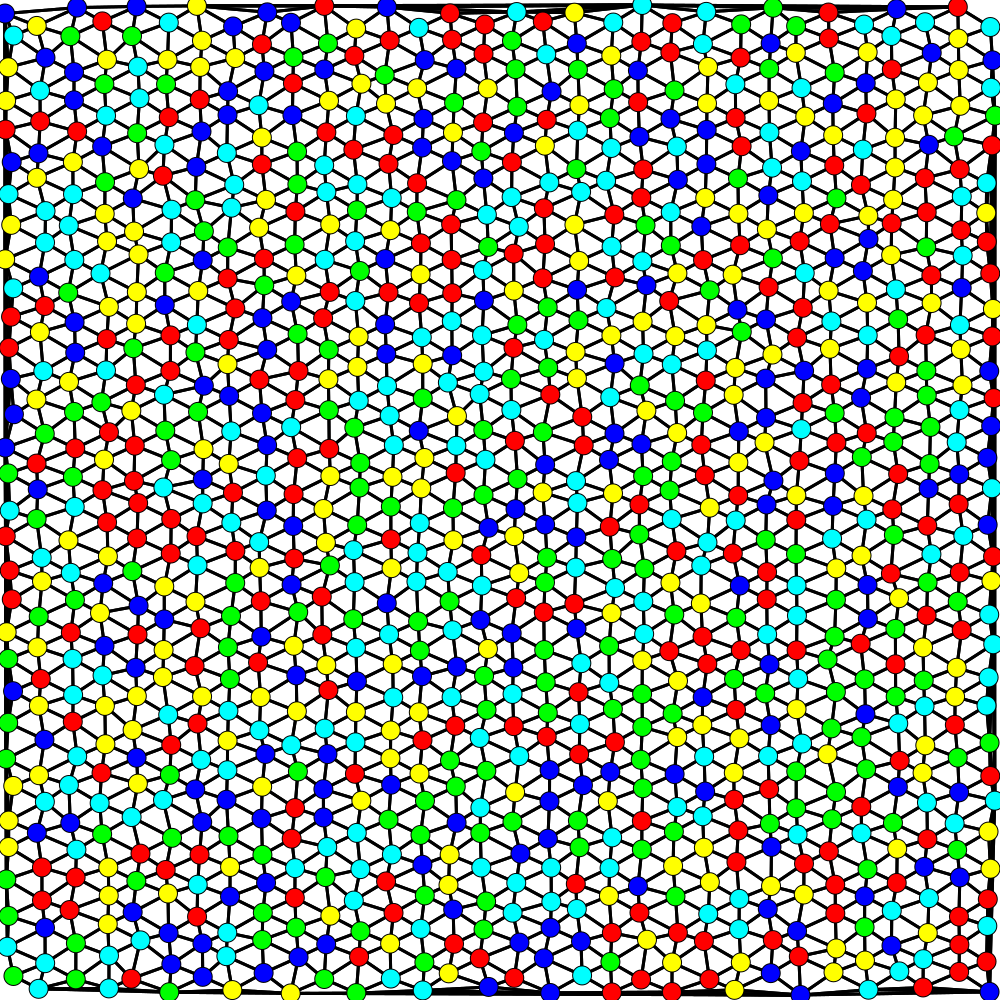
\includegraphics[width=\textwidth]{img/partitioning_false.png}
\caption{Non-partitioned graph.}
\end{subfigure}
~
\begin{subfigure}[b]{0.48\textwidth}
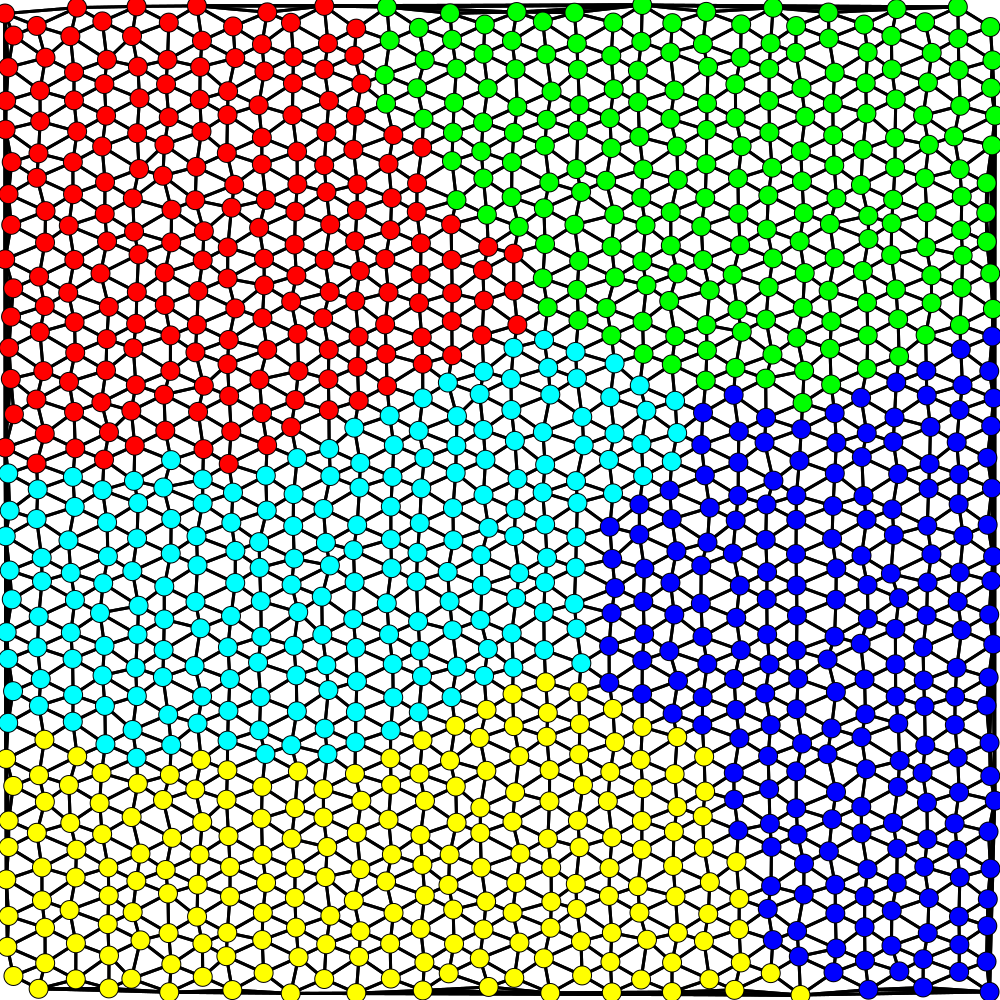
\includegraphics[width=\textwidth]{img/partitioning_true.png}
\caption{Partitioned graph.}
\end{subfigure}
\caption{Figure shows the difference in number of overlapping edges in between threads for non-partitioned and partitioned graphs. Each color represents nodes belonging to different threads.}
\label{fig:partitioning}
\end{figure}
